\documentclass[a4paper,twocolumn]{article}
\usepackage{booktabs}
 \usepackage[pdftex]{graphicx}   
\usepackage{subfig}
\usepackage{amsmath}
\newcommand{\BigO}[1]{\ensuremath{\operatorname{O}\bigl(#1\bigr)}}
\title{Efficient Construction of Non-Transitive Dice}
\author{Stephen I. Roberts}
\date{\today}
\begin{document}
	\maketitle
	\begin{abstract}
		Efron's dice are a set of four six-sided dice labelled A-D with the unusual feature that dice A beats B, B beats C, C beats D and D beats A with probability $p=\frac{2}{3}$ when rolled. This paper investigates general systems of $m$
dice each with $n$ sides which exhibit this property of non-transitive dominance.
We present an asymptotically efficient algorithm able to generate sets of maximally non-transitive dice for arbitrary values of $m$ and $n$.
Our approach allows the construction of sets which are of magnitude larger than was previously possible. This work is also relevant to the study of cyclic majority paradoxes within voting systems.
	\end{abstract}
	
	\section*{Introduction}
	Consider a two player dice game in which the winner is the person who manages to roll the highest score using dice with a non-standard numbering system. The first player takes one dice from a set and rolls it. The second player then repeats this process, choosing from the remaining untouched dice. Intuitively, one expects games of chance such as this to either favour the first player if the dice are numbered so that one dice strictly dominates all others, or to be evenly matched otherwise. In fact, as noted by Bradley Efron and subsequently popularized by Gardner \cite{gardner1970non}, this is not necessarily the case. It is possible to construct sets of dice such that regardless of the selection made by the first player, the second is likely to win the game.
	

Efron's dice were developed by Bradley Efron, a statistician at Stanford University, to illustrate a general class of probability paradoxes which violate transitivity. \tablename~\ref{tab:efrons:face} shows these dice, and a quick inspection confirms that each dice will beat its successor in $\frac{2}{3}$ of all possible pairwise results. In fact, this is the greatest possible advantage one can achieve for a system of six-sided dice \cite{gardner2001colossal}.

\begin{table}
\begin{center}

\subfloat[Dice Faces]{
	\begin{tabular}{|c|c|c|c|} 
	\hline
	a & b & c & d  \\ 
	\hline

 3 & 6 & 5 & 4 \\
 3 & 6 & 5 & 4 \\
 3 & 2 & 5 & 4 \\
 3 & 2 & 1 & 4 \\
 3 & 2 & 1 & 0 \\
 3 & 2 & 1 & 0 \\
 
 	\hline
	 \end{tabular} 
	 \label{tab:efrons:face}
	 }
	 \qquad
	 \subfloat[Advantage Table]{
	\begin{tabular}{|c|c|c|c|} 
	\hline
	a & b & c & d  \\ 
	\hline
 4 & 6 & 6 & 6 \\
 4 & 6 & 6 & 6 \\
 4 & 3 & 6 & 6 \\
 4 & 3 & 2 & 6 \\
 4 & 3 & 2 & 0 \\
 4 & 3 & 2 & 0 \\
 	\hline
	 \end{tabular} 
	 	 \label{tab:efrons:dom}
	 }
	 
\end{center}
\caption{Different Representations of Efron's Dice}
\end{table}
This paper contributes a general method for constructing systems of non-transitive dice of arbitrary size with the greatest possible mutual advantage. We build on work by Tenney{\it et al.}~\cite{tenney1976non} which provides key insights into the algorithmic construction of such dice. Their approach relies on searching a space of possible dice rather than directly constructing them, and therefore is limited by the combinatorical explosion of candidate sets. Conversely, our approach allows the direct construction of non-transitive dice in \BigO{m\times n} time where $m$ is the number of dice and $n$ is the number of sides per dice. This is trivially asymptotically efficient as it is impossible to beat this bound whilst still outputting a set of dice with $m\times n$ total face values.

\section*{Dice Construction}
There are infinitely many ways to number a set of dice given complete freedom to choose face values from the set of all integers. To make this problem tractable, limits must be applied to the numbers we can choose. Approaches to this problem tend to begin by applying heuristics to limit the search space. A simple example would be to constrain ourselves to choosing values between $[1 .. n\times m]$ which guarantees a finite, albeit massive, search space whilst still allowing for any possible ordering of faces.

Arguably the most powerful heuristic yet devised is the advantage table described by Tenney{\it et al.}~\cite{tenney1976non}. This abstracts away face values in favour of the relative orderings of faces. At a high level, an advantage table simply shows the number of faces on dice $d+1$ dominated by the faces on dice $d$. \tablename~\ref{tab:efrons:dom} shows the advantage table constructed from the set of Efron's Dice shown in \tablename~\ref{tab:efrons:dom}. More formally, given dice matrix $D$, advantage matrix $A$, dice $d$ and face $f$ then: 
\begin{equation}
A_{d,f} = \sum\limits_{i=1}^n \begin{cases}
1 &\text{if $D_{d,f}>D_{d+1, i}$}\\
0 &\text{otherwise}
\end{cases}
\end{equation}

This technique is beneficial because it reduces the search space by collapsing equivalence classes which have the same relative orderings but different numberings into a single representation. That said, is only useful if we can reverse the procedure and construct sets of dice from their advantage tables. Tenney{\it et al.}~\cite{tenney1976non} show that this is possible if and only if the advantage table corresponds to a feasible set of dice. To put it another way, for every set of non-transitive dice there is a corresponding advantage table which uniquely describes it. They use this fact to construct sets of dice by iterating through the possible advantage tables and attempting to construct sets of dice from them. When this construction succeeds, then an optimal set of non-transitive dice has been found.

Whilst this approach improves on naive searches it still suffers from a combinatorial explosion in the size of the search space, limiting discovery to dice not much larger than 20 sides. Conversely, our approach allows us to directly generate advantage tables which will correspond to optimal dice sets.



\subsection*{Dice Numbering}

Although there is already an algorithm detailed in~\cite{tenney1976non} for converting advantage tables to systems of numbered dice, it is instructive to consider this problem as an intermediary step towards dice construction.

The advantage table representation has a number of important properties which we must consider before continuing. Firstly, we always represent dice sets, and therefore advantage tables, in a sorted fashion with the highest value at the top by convention. This prevents us from wasting time considering cyclic permutations of dice faces which are equivalent given we assume all faces can be rolled with equal probability on a fair dice. Secondly, the summation of one column of an advantage table represents the number of instances in which the corresponding dice beats its successor out of the $n^2$ possible outcomes. Inspecting \tablename~\ref{tab:efrons:dom} we see that in the case of Efron's Dice each column sums to 24, meaning the dominating player will win in $\frac{24}{36}$ cases, i.e. $p=\frac{2}{3}$.

We can interpret the advantage table of an optimal set of non-transitive dice as a directed acyclic graph (DAG). In this representation, nodes represent individual dice faces and edges the dominance relations which exist between them. For example, if $A_{d,f}=3$, we have edges $\lbrace A_{d,f} \rightarrow A_{d+1, 1},A_{d,f} \rightarrow A_{d+1, 2},A_{d,f} \rightarrow A_{d+1, 3}\rbrace$. Edges only exist between consecutive dice and always travel in the direction of dominance. The graph must be acyclic due to the transitive property of the greater than relation on integer numbers. If any cycles exist in this representation, we are claiming that $\exists d,f :  A_{d,f} >  A_{d,f}$, meaning this is not a valid advantage table.

Now that we have shown we can represent our advantage table as a DAG, assigning numbers to faces becomes analogous to a topological sorting of this DAG. By definition there must be a non-empty set of dice faces corresponding to minimal elements in the graph, so we assign the value of zero to these faces and delete the corresponding vertices. This procedure is repeated with incrementing labels until we run out of vertexes. On termination all faces will have been numbered and hence we will have constructed a system of non-transitive dice. This algorithm is far from optimal and should not be used in practice, but it lays the groundwork for how we may generate advantage tables.

\subsection*{Advantage Table Construction}

The correspondence between valid advantage tables and directed acyclic graphs forms the basis of our algorithm. Assuming we can derive the maximal mutual beating probability of a system of dice it is a trivial matter to convert this value to the sum of each column of its advantage table by multiplying it by $n^2$. This calculation is mentioned in \cite{tenney1976non}, but a full derivation will be presented later in this paper. For now, let this value be represented by $s$. Formally, 
\begin{equation}
\forall x \in [1..m], \sum\limits_{i=1}^n A_{x,i} = s
\end{equation} 


\begin{table}
\begin{center}


	\begin{tabular}{|r|c|c|c|c|} 
	\hline
	Face & a & b & c & d  \\ 
	\hline\hline

 6& 4 &   &   &   \\ \hline
 5&  &   &   &   \\ \hline
 4&  & 3 &   &   \\\hline
 3&  &   &  2 &   \\\hline
 2&  &   &   & 0  \\\hline
 1&  &   &   &   \\
 
 	\hline
 	
	 \end{tabular} 

\end{center}
\caption{Top cycle construction for Efron's Dice}
\label{tab:toppath:efron}
\end{table}



In order to ensure that our advantage table corresponds to a DAG it is constructed via a further intermediate representation we call the `top path'. This can be thought of as a slowest-decent path through the DAG. We construct this iteratively by starting at the most dominant vertex on the first dice and numbering this with the lowest possible value $v$ which still allows the corresponding column to sum to $s$. The next vertex chosen is then vertex $v$ on the second dice. Again this is given the lowest possible number whilst maintaining the property that $\sum\limits_{i=1}^n A_{2,i} = s$. This process continues until this path reaches a minimal vertex on the DAG. 

This process is best understood with a worked example. We start at the top-left of the advantage table, at $A_{a,6}$. This column has to sum to $24$, which can only be done if $A_{a,6} \geq \lceil24\div6\rceil = 4$. This is because  $A_{a,[1..5]}$  have to be less than or equal to $A_{a,6}$ due to our ordering and the fact that $6 \times 3 < 24$. As we are trying to minimize its value, we choose $A_{a,6}=4$. We now move on to the 4th cell for the next dice in sequence, $A_{b, 4}$. In this instance, we have two unconstrained cells above us, $A_{b,6}$ and $A_{b,5}$. Let us therefore assume then that these cells hold the maximum possible value, i.e. $A_{b,6} = A_{b,5} = 6$ for 6-sided dice. This leaves a deficit of $12$ which need to be accounted for by cells $A_{b,1..4}$. We therefore set $A_{b,4} = \lceil12\div4\rceil=3$. The same logic yields $A_{c,3}=\lceil6\div3\rceil = 2$ and $A_{d,4}=\lceil0\div2\rceil=0$. \tablename~\ref{tab:toppath:efron} gives the results of this process in tabular form.

It is trivial to convert from this top path representation to a full advantage table by starting at the top of each column and assigning the maximum possible value to each empty cell in turn. Cells above, and therefore unconstrained by, the top path are assigned to be the minimum of $n$ and the remaining dominance yet to be accounted for. Those below, and thereby constrained by, the top path are numbered as the minimum of the value within the top path cell and the remaining dominance yet to be accounted for. Given the remaining dominance decreases as we attribute dominance values to cells we know that the values in a column will appear in descending order.

The reason we start by constructing the top path is that it guarantees an acyclic DAG for the advantage table. If a cycle did exist for the advantage table it would have to cross over the top path at some point given the latter traverses the entire height of the table. This is a contradiction, however, as it would require some cell in the advantage table to have higher dominance than a top-cycle element above it, which is impossible as the elements in each column are guaranteed to be in descending order.
\def\app#1#2{%
  \mathrel{%
    \setbox0=\hbox{$#1\sim$}%
    \setbox2=\hbox{%
      \rlap{\hbox{$#1\propto$}}%
      \lower1.1\ht0\box0%
    }%
    \raise0.25\ht2\box2%
  }%
}
\def\approxprop{\mathpalette\app\relax}
\subsection*{The Odds}
So far we have shown how to construct optimal non-transitive dice when given the corresponding values for $m$ dice, $n$ sides and mutual dominance $s$. This section will describe how we can derive suitable values for these parameters and hence construct arbitrary sets of non-transitive dice.

    \begin{figure}[ht]
    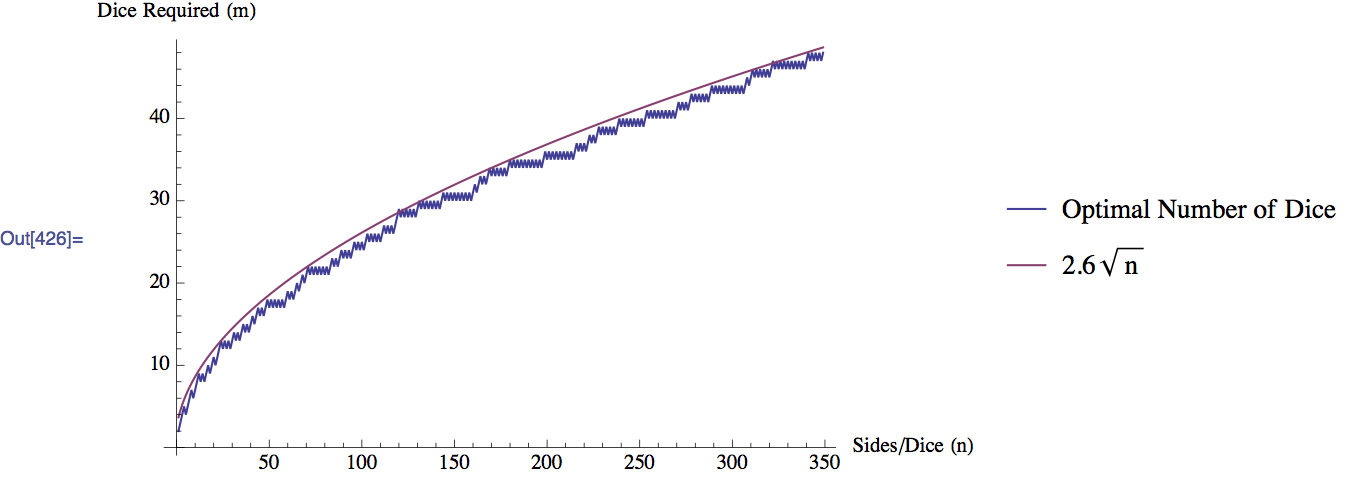
\includegraphics[width=\linewidth]{DicePlot}
    \caption{Dice in Optimal Configurations}
    \label{fig:graph}
    \end{figure}
 
The first thing to note is that the precise number of dice in a set is not as important as it at first appears. Too small a value of $m$ relative to the choice of $n$ will limit the mutual beating probability, but above a certain limit additional dice will confer no further benefit. The reason for this can be seen in the top path construction algorithm which simply assumes it can use as many dice as required to generate an optimal set for a given $s$. This algorithm always generates optimal paths of minimal finite length, which experiments show to be $m \approxprop 2.6\sqrt{n}$ as shown in \figurename~\ref{fig:graph}. Given our algorithm does not require a value for $m$ to function, we choose to ignore it. If a tight constraint is required on the value of $m$, our method can be modified to allow the top path algorithm to wrap around back on itself. This is left as an excercise to the reader.

Any algorithm to generate sets of dice must be allowed some input to function. We choose to generate sets of dice for a given number of sides per dice. We therefore expect the value of $n$ to be specified. This only leaves the value of $s$ to be calculated. We use a variant of the derivation provided in \cite{tenney1976non} to show that we can produce a value for s with equation 4 below.

\fbox{
 \begin{minipage}{\textwidth}\textbf{Marker's Comments} \hfill \vspace{2in}
\end{minipage} 
}



\begin{equation}
P(n) = \frac{6n^2 -4n +(-1)^n -1}{8n^2}
\end{equation}
\begin{equation}
S(n) = n^2\cdot P(n) = \frac{6n^2 -4n +(-1)^n -1}{8}
\end{equation}
\section*{Conclusion}

\bibliographystyle{plain}
\bibliography{cites}
\end{document}
